\documentclass[10pt]{article}
\usepackage[margin=2cm]{geometry}
\usepackage{amsmath,amssymb}
\usepackage{booktabs}
\usepackage{graphicx}
\usepackage{float}
\usepackage[font=small,labelfont=bf]{caption}
\usepackage[compact]{titlesec}
\usepackage{enumitem}
\usepackage{microtype}
\usepackage[hidelinks]{hyperref}
\setlist{itemsep=1pt,topsep=3pt}
\setlength{\parskip}{4pt}
\setlength{\parindent}{0pt}
\graphicspath{{figures/}}
\newcommand{\fig}[1]{Figure~\ref{#1}}
\newcommand{\tab}[1]{Table~\ref{#1}}

\begin{document}
\sloppy

\begin{center}
{\LARGE SuperMimic on Kangaroo, M3: imagination and the policy update}\\[4pt]
The code of the online loop, checked on the frozen M2 world model. Branch \texttt{omm/supermimic} of
pal\_mjlab, 23 October 2026.
\end{center}

\section*{Summary}

M3 built the policy-update code of SuperMimic and checked it on the frozen M2 world model. Built:
\begin{itemize}
  \item the analytic heads (reward, observation, goal, critic input);
  \item the online replay buffer;
  \item imagination with the survival weight (paper Eq.~2) and the critic's $\lambda$-returns (Eq.~3);
  \item the full training loop (Alg.~A.1) as an mjlab runner.
\end{itemize}
The checks use the PPO-Sim actor (the same network) with replay states of that same policy.

\begin{itemize}
  \item \textbf{Imagination reproduces the simulator in closed loop.} From 1024 held-out starts the
  actor's imagined 32-step return is within \textbf{0.9\%} of the simulated one. The two correlate at
  0.995 across starts, and body positions differ by 2.1\,cm after 32 steps.
  \item \textbf{The BPTT gradient improves the real return.} Without the critic, 300 updates raise the
  simulated 32-step return by \textbf{7\%}, with imagination within 0.4\% throughout.
  \item \textbf{On a frozen model the policy does not hold on whole clips.} In every run the paper's
  benchmark degrades:
  \begin{itemize}
    \item without the critic, the objective is myopic: 829 of 1296 clips fail (26 at the start);
    \item with the critic at the paper's learning rate, 406--415 clips fail;
    \item with a $10\times$ smaller step, 83 clips fail.
  \end{itemize}
  The frozen learned failure head also missed the new policy's falls (0.4\% predicted vs 8.3\% in the
  simulator). The paper never trains on a frozen model; its online refits are meant to prevent exactly
  this, so M4 must watch it.
  \item \textbf{Ready for M4.} The training task runs with mjlab's normal CLI in three
  configurations: \texttt{dev} locally in bf16, and \texttt{dev} and \texttt{full} on a cluster with
  the paper's settings. Locally an iteration takes 1.57\,s and 11.3\,GB. The motion data sit in one
  transferable folder, with the training libraries downloadable from the motion browser.
\end{itemize}


\section{What M3 is for}

\textbf{The update being checked.} SuperMimic improves the policy by imagining $H = 32$ steps with
the world model from replay states and backpropagating the imagined return (paper Eq.~2):
\[
J(\theta) = \sum_{t=0}^{H-1} \gamma^t c_t\, \hat r_{t+1} + \gamma^H c_H\, V(\hat s_H),
\qquad c_{t+1} = c_t\,(1 - \hat d_{t+1}).
\]
\begin{itemize}
  \item The critic $V$ is fit to $\lambda$-returns of the same imagined rollouts (Eq.~3).
  \item The world model is refit every iteration on fresh simulator data (Alg.~A.1).
\end{itemize}

\textbf{Why a short check, not a frozen-model training run.} The paper never trains a policy on a
frozen model; its refits are what stop the policy from exploiting model errors. M3 therefore checks
the code that M4 runs, where the M2 model knows the data: the PPO-Sim actor (same network as the
SuperMimic policy, D17) and replay states of that same policy. Every comparison between methods is
left to the online loop (M4).

\textbf{Two checks.}
\begin{enumerate}
  \item \textbf{Closed loop, no training.} The actor acts 32 steps in imagination and in the
  simulator from the same 1024 held-out starts. Does imagination reproduce the simulator when the
  policy reacts to imagined observations?
  \item \textbf{A short update run.} Fit the critic with the actor fixed, then run 300 policy
  updates. Do the gradients, the clipping and the critic fit work, and what happens to the policy in
  the simulator?
\end{enumerate}

\section{What was built}

\subsection{Analytic heads}

The paper's world model has a learned dynamics model and reward, observation and termination heads,
``each either learned or computed analytically''. Our dynamics and termination head are the M2
networks. The reward $\hat r$, the noise-free observation $\hat{\bar o}$ and the goal are computed from
the predicted state with forward kinematics and the training env's own definitions (D5, D32):
\begin{itemize}
  \item \textbf{Reward:} every reward term of the env (Table~A.2): the six tracking terms, the action
  rate and the joint-limit penalty, with the env's weights, widths and $\times\,dt$.
  \item \textbf{Observation} (Table~A.1): $q - q_0$ with the calibration offset of $\xi$, $\dot q$,
  IMU angular velocity and projected gravity (from the IMU site's kinematics), and the previous
  action, in a 10-frame history. Sensor noise is added back as in the paper.
  \item \textbf{Goal and critic input:} the next 10 reference frames, and $(\hat s, g, \xi)$ plus the
  privileged root-pose error and time left (D7).
  \item \textbf{Failure rule} (for comparison with the learned head, D31) and the clip end (D8).
\end{itemize}
An env term without an analytic head raises an error, so imagination never silently optimizes a
different objective.

\textbf{Parity.} Along random-action rollouts with episode ends and resets, the heads evaluated on the
true states match the env: goal and critic input to $10^{-4}$, the full 10-frame proprioceptive
history to $10^{-4}$, the reward to $10^{-5}$, and the failure and clip-end flags exactly.

\subsection{Replay buffer, imagination and updates}

\begin{itemize}
  \item \textbf{Replay} (Alg.~A.1, D9, D33): a FIFO of 1000 rows per env. A transition row holds a
  state and the executed noisy action; an episode's terminal state is an extra row without an action.
  Windows for Eq.~1 are $k$ consecutive transition rows plus the next row, so they never span two
  episodes. Imagination starts come with their previous 9 rows, which are turned into the policy's
  observation history.
  \item \textbf{Imagination} (\texttt{imagine}): Eq.~2 with the survival weight from the learned head
  or the rule (one switch), clip ends handled as in D8, the failure rule computed alongside.
  \item \textbf{Updates} with the paper's settings (Table~A.5):
  \begin{itemize}
    \item world model: 10 batches of 2048 windows, $k = 8$;
    \item policy: 4096 rollouts, Adam $\beta = (0.9, 0.95)$, gradient clip at global norm 1.0 then
    0.1 per element, the world model and critic frozen;
    \item critic: $\lambda = 0.95$, 5 epochs of 4 minibatches, targets fixed per rollout;
    \item all learning rates $2\cdot10^{-4}$ with the cosine decay to $0.03\times$ over 250k
    iterations.
  \end{itemize}
\end{itemize}

\textbf{Tests} (CPU, tiny library): $\lambda$-returns against their limits ($\lambda = 0$: one-step
targets; $\lambda = 1$: the bootstrapped discounted sum); the policy-objective gradient through the
whole imagination against finite differences; the policy step leaves the world model and the critic
untouched; replay windows and histories on a synthetic stream with wraparound; and an end-to-end run
of the training loop with checkpoint and resume.

\subsection{The online loop and the mjlab CLI}

The M4 loop is an mjlab runner (\texttt{SuperMimicRunner}), registered with the tasks
\texttt{Mjlab-SuperMimic-Flat-Pal-Kangaroo-Grippers} and \texttt{...-ArmWaist1Hz}. mjlab's \texttt{train}
and \texttt{play} drive it on any machine with mjlab; every setting is a CLI flag. Each iteration
collects about 2.5 environment steps (UTD 0.4), fits the world model, and runs one policy and critic
update. Besides the losses it logs:
\begin{itemize}
  \item the imagined vs simulated 32-step return of the current policy from the same states;
  \item how the learned failure head and the env's rule rank fresh simulator failures (D31).
\end{itemize}
The motion data are chosen on the command line (D35): a dataset folder, possibly relative, and a
subset (\texttt{dev}, \texttt{full} or a number of hours), packed on first use.

\section{Check 1: imagination in closed loop}

\textbf{Protocol.} 1024 starts from held-out clips of the PPO-Sim policy's replay data. The simulator
is put in each start state with its $\xi$ and reference frame, and its observation history is
backfilled with the start frame. Imagination starts from the same state and the same observation
tensor. Neither side has sensor or action noise. The actor then acts 32 steps on each side.

\begin{table}[H]
\centering\small
\caption{Check 1: the PPO-Sim actor in the simulator and in imagination, from the same 1024 held-out
starts. Return: discounted reward sum over 32 steps, until a failure or clip end.}
\label{tab:check1}
\begin{tabular}{lrrr}\toprule
 & 32-step return & gap & failures \\\midrule
simulator & 1.869 &  & 0.49\% \\
imagination, learned head & 1.852 & $-0.9$\% & 0.40\% \\
imagination, env's rule & 1.852 & $-0.9$\% & 0.56\% \\
\bottomrule\end{tabular}

\end{table}

\begin{figure}[H]
\centering
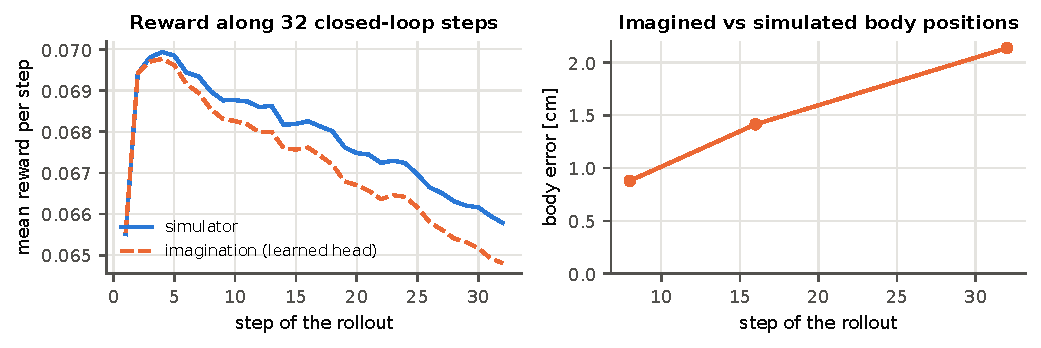
\includegraphics[width=\textwidth]{check1.pdf}
\caption{Check 1. Left: mean reward per step in the simulator and in imagination (weighted by the
imagined survival). Right: body positions of the imagined vs the simulated rollout, relative to the
root, after 8, 16 and 32 steps.}
\label{fig:check1}
\end{figure}

\begin{itemize}
  \item \textbf{Returns agree:} $-0.9\%$, with correlation 0.995 across starts. Imagination is slightly
  pessimistic, and the gap grows along the rollout (\fig{fig:check1}).
  \item \textbf{Failures agree:} 0.49\% in the simulator, 0.40\% predicted by the learned head, 0.56\%
  by the rule.
  \item \textbf{States agree:} the imagined body positions are 0.9, 1.4 and 2.1\,cm from the simulated
  ones after 8, 16 and 32 steps. In M2 the open-loop error on logged actions was 0.9, 1.7 and 3.8\,cm;
  in closed loop the policy corrects part of the drift.
\end{itemize}

This exercises everything the policy sees and is scored on in imagination: the observation head
and history, the goal, the reward, the termination and the clip-end handling. All of it behaves like
the simulator.

\section{Check 2: policy updates on the frozen model}

\textbf{Protocol.}
\begin{enumerate}
  \item \textbf{Critic first.} 200 iterations fit only the critic, with the actor fixed. Its loss falls
  from 0.29 to 0.043, and the value at the start matches its $\lambda$-return target (5.13,
  \fig{fig:critic}).
  \item \textbf{Updates.} 300 policy updates with the paper's settings (Table~A.5), from starts on the
  training clips.
  \item \textbf{Evaluation.} Check~1 every 50 updates, plus the paper's benchmark (every \texttt{dev}
  clip once from its first frame, no randomization) at the start and the end.
  \item \textbf{Variants.} Three more runs change one thing each: no critic (the paper's ablation),
  policy learning rate $2\cdot10^{-5}$ (PPO-Sim's final rate; the paper's $2\cdot10^{-4}$ is meant
  for training from scratch), and the env's failure rule as the termination (D31).
\end{enumerate}

\begin{table}[H]
\centering\small
\caption{Check 2: the policy before and after 300 updates on the frozen model. Benchmark: every
\texttt{dev} clip from its first frame. Closed loop: check~1 after the last update. Worst gap: the
largest imagined-vs-simulated return gap over the evaluations.}
\label{tab:update}
\setlength{\tabcolsep}{4pt}
\resizebox{\textwidth}{!}{\begin{tabular}{lrrrrrr}\toprule
 & \multicolumn{3}{c}{benchmark (1296 clips)} & \multicolumn{3}{c}{closed loop, 32 steps} \\
\cmidrule(lr){2-4}\cmidrule(lr){5-7}
policy & failed & tracking return & arms [cm] & return & failures & worst gap \\\midrule
PPO-Sim actor (start) & 26 & 0.742 & 10.8 & 1.869 & 0.5\% & \\\midrule
after 300 updates, paper settings (learned head, critic, lr $2\cdot10^{-4}$) & 415 & 0.465 & 19.4 & 1.778 & 0.4\% & 25.3\% \\
after 300 updates, without the critic & 829 & 0.534 & 8.9 & 2.003 & 0.7\% & 0.4\% \\
after 300 updates, policy learning rate $2\cdot10^{-5}$ & 83 & 0.673 & 12.5 & 1.869 & 0.6\% & 0.4\% \\
after 300 updates, termination by the env's rule & 406 & 0.500 & 16.1 & 1.835 & 0.3\% & 0.8\% \\
\bottomrule\end{tabular}
}
\end{table}

\begin{figure}[H]
\centering
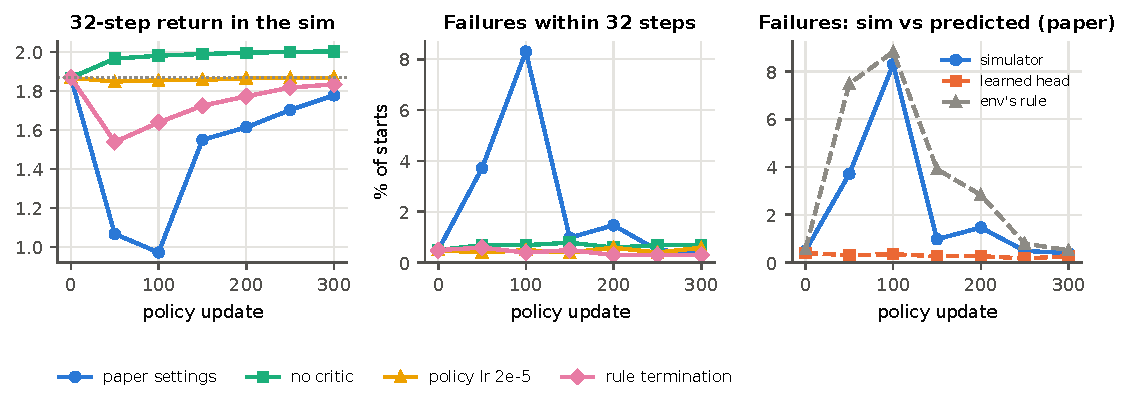
\includegraphics[width=\textwidth]{update.pdf}
\caption{Check 2, closed loop every 50 updates. Left: simulated 32-step return (dotted: the start).
Middle: share of starts failing within 32 steps. Right, paper settings: failures in the simulator vs
those predicted by the learned head and by the rule.}
\label{fig:update}
\end{figure}

\begin{figure}[H]
\centering
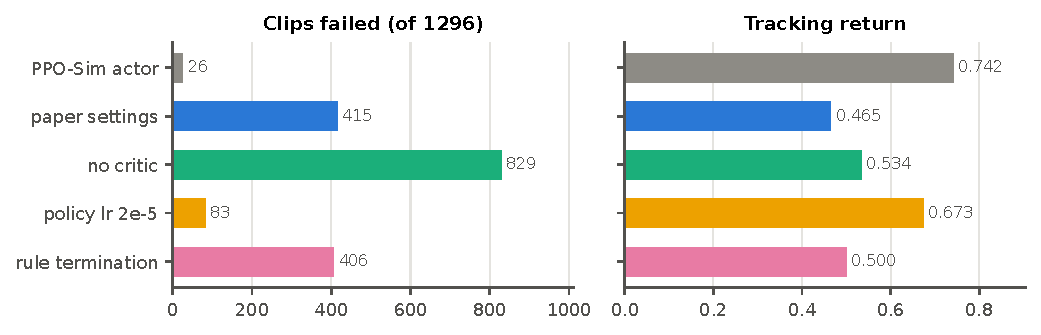
\includegraphics[width=0.9\textwidth]{benchmark.pdf}
\caption{The paper's benchmark (1296 \texttt{dev} clips, each from its first frame) before and after
300 updates on the frozen model.}
\label{fig:benchmark}
\end{figure}

\textbf{What works.}
\begin{itemize}
  \item \textbf{The update improves what it optimizes.} Without the critic the objective is the
  imagined 32-step return. 300 updates raise the \emph{simulated} 32-step return from 1.869 to 2.003
  (+7\%), and the arm error on whole clips falls from 10.8 to 8.9\,cm. This is the policy-level
  version of M2's gradient check.
  \item \textbf{Imagination keeps up with a changing policy.} In every run the imagined and simulated
  closed-loop returns stay within 1\%, except at the trough of the paper run.
  \item \textbf{The critic tracks its targets} throughout (\fig{fig:critic}), the clipping keeps the
  gradient norm near 1 once training settles, and the world model and critic stay frozen in the
  policy step (tested).
\end{itemize}

\textbf{What fails, and why.}
\begin{itemize}
  \item \textbf{The 32-step objective is myopic.} Without the critic the policy tracks better in the
  short run but loses balance later: 829 clips fail. A fall after step 32 never enters the objective.
  This is the paper's argument for the critic.
  \item \textbf{On a frozen model, the critic misjudges the long run.} With the critic at the paper's
  learning rate, 406--415 clips fail.
  \begin{itemize}
    \item The critic's values come from imagined rollouts of states near the old policy. No falls of
    the new policy ever come back from the simulator to correct it.
    \item With a $10\times$ smaller step the policy moves less and the damage is smaller (83 clips),
    but it is still there.
  \end{itemize}
  \item \textbf{The frozen learned head missed the new policy's failures.} In the paper run the
  simulated failure rate climbed to 8.3\% of starts at update 100. The head kept predicting about
  0.4\%; the rule predicted 8.8\% (\fig{fig:update}, right).
  \begin{itemize}
    \item With falls free in imagination, the critic's values inflated from 5.1 to 7.9, and the 32-step
    return dipped to 0.97 before recovering.
    \item With the rule as termination, the dip is much milder (1.54) and failures stay under 0.6\%.
    \item But the whole-clip damage is the same (406 clips): the head explains the transient, not the
    long-run loss.
  \end{itemize}
\end{itemize}

\begin{figure}[H]
\centering
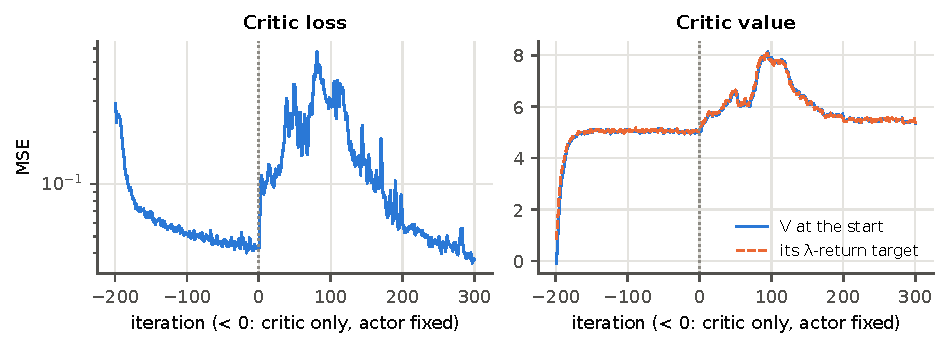
\includegraphics[width=0.85\textwidth]{critic.pdf}
\caption{Critic of the paper run. Iterations below 0 fit only the critic (actor fixed); from 0 on the
policy is updated too. Right: the value of the start states and its $\lambda$-return target.}
\label{fig:critic}
\end{figure}

\textbf{Reading.} These are the failure modes the paper's loop is built against. In Alg.~A.1, the
simulator data of the current policy keep flowing into the replay. Its falls are refit into the world
model, and from there they reach the imagined rollouts, the termination head and the critic. M3 froze
all of that on purpose. The online loop is only tested in M4, which must watch for these symptoms
(Section~\ref{sec:m4}).

\textbf{Gate.}
\begin{itemize}
  \item Check 1 passes.
  \item The update machinery passes: gradients against finite differences, the critic fit, clipping,
  frozen parameters, and imagination tracking the simulator.
  \item ``The simulated return holds'' passes over 32 steps (no critic, small step) but fails on whole
  clips in every frozen-model run.
\end{itemize}
We see no sign of a code defect in that failure. Its causes are identified, and they are the reason
the paper refits online.

\section{Ready for M4}
\label{sec:m4}

\textbf{Launch.} The task \texttt{Mjlab-SuperMimic-Flat-Pal-Kangaroo-Grippers-ArmWaist1Hz} runs with
mjlab's \texttt{train} CLI on any machine. The commands are in \texttt{docs/supermimic/README.md}.
\begin{itemize}
  \item \textbf{\texttt{dev}, local 16\,GB GPU:} bf16 learning updates and a replay of 500 steps per
  env (D16). The paper settings ran out of memory locally: TF32 imagination needs about 12.7\,GB plus
  the simulator and the replay.
  \item \textbf{\texttt{dev} and \texttt{full} on a cluster:} the paper's settings (TF32, replay 1000).
  The \texttt{full} library (124,079 clips, 250.9\,h) is packed and takes 13.9\,GB on the GPU.
  \item \textbf{Data:} \texttt{--env.commands.motion.dataset <path>} (relative paths allowed) and
  \texttt{--env.commands.motion.subset dev|full|10h}.
  \begin{itemize}
    \item The dataset folder \texttt{kangaroo\_bones\_seed/dataset/} holds the retargeted motions
    (\texttt{motions/}, \texttt{.pkl}), the training libraries (\texttt{libraries/<subset>/}) and the
    manifest.
    \item rsync it, or download it from the motion browser (motions zip, or each library file,
    resumable).
  \end{itemize}
  \item \textbf{Resume} after a preemption: \texttt{scripts/supermimic/train.py} with the same
  arguments continues the newest checkpoint of runs with the same run name.
\end{itemize}

\begin{table}[H]
\centering\small
\caption{Local smoke run of the M4 task from scratch (RTX 5060 Ti, \texttt{dev}, bf16, replay 500,
60 iterations).}
\label{tab:smoke}
\begin{tabular}{lr}\toprule
collect (2.5 env steps) & 0.15 s \\
world model (10 $\times$ 2048 windows) & 0.31 s \\
policy and critic (4096 rollouts $\times$ 32 steps) & 1.11 s \\\midrule
iteration & 1.57 s (2,298 per hour) \\
peak GPU memory & 11.3 GB \\
\bottomrule\end{tabular}

\end{table}

\textbf{Smoke run.} 60 iterations from scratch work end to end: collection, world-model fit, policy
and critic updates, evaluation, checkpoint and benchmark. About 2,300 iterations per hour means a
12\,h local run reaches about 27k of the paper's 320k iterations. Early signals:
\begin{itemize}
  \item the imagined vs simulated 32-step return is already within $-5$\ldots$+2\%$;
  \item the learned head's AUC on fresh failures rose from 0.42 to 0.81 within 60 iterations of
  online refits, with the rule at 1.0, as hoped when choosing the learned head (D31).
\end{itemize}

\textbf{What M4 must watch,} given M3:
\begin{itemize}
  \item \textbf{Simulator episodes:} failures and length (\texttt{episode/*}).
  \item \textbf{Imagination vs simulator:} the return gap (\texttt{eval/return\_gap\_head}).
  \item \textbf{The learned head vs the rule:} AUC on fresh failures (\texttt{termination/*}), and
  predicted vs simulated failures (\texttt{eval/imagined\_failure\_head} vs
  \texttt{eval/sim\_failure}).
  \item \textbf{The whole-clip benchmark} of the saved checkpoints (\texttt{eval.py}). The 32-step
  checks cannot see falls that happen later.
\end{itemize}

\appendix
\section{Settings and reproduction}

\textbf{Check settings:}
\begin{itemize}
  \item paper settings throughout (Table~A.5): 4096 rollouts, $H = 32$, Adam $\beta = (0.9, 0.95)$,
  clip 1.0 then 0.1, $\lambda = 0.95$, 5 epochs $\times$ 4 minibatches, learning rates
  $2\cdot10^{-4}$;
  \item bf16 learning updates (D16);
  \item replay: the PPO-Sim iteration-8800 data of M2 (4096 envs $\times$ 500 steps).
\end{itemize}
Each run takes 10--14 minutes on the local GPU (peak 11.5\,GB) including two benchmarks.

\begin{footnotesize}
\begin{verbatim}
python -m pal_mjlab.scripts.supermimic.m3_check --out-json logs/supermimic_m3/m3.json
#   variants: --no-use-critic --critic-iterations 0 | --actor-lr 2e-5 | --termination rule
python docs/supermimic/m3/make_figures.py && (cd docs/supermimic/m3 && latexmk -pdf report.tex)
# M4 smoke (local): mjlab's train CLI
train Mjlab-SuperMimic-Flat-Pal-Kangaroo-Grippers-ArmWaist1Hz --agent.max-iterations 60 \
  --agent.algorithm.precision bf16 --agent.replay-steps 500 --agent.run-name smoke-local-bf16
\end{verbatim}
\end{footnotesize}

\textbf{Code.}
\begin{itemize}
  \item In \texttt{src/pal\_mjlab/tasks/supermimic/rl/}: \texttt{heads.py}, \texttt{replay.py},
  \texttt{supermimic.py}, \texttt{runner.py}.
  \item In \texttt{scripts/supermimic/}: \texttt{m3\_check.py} and the resumable \texttt{train.py}.
  \item Tests in \texttt{tests/supermimic/}: \texttt{test\_heads.py}, \texttt{test\_replay.py},
  \texttt{test\_supermimic.py}, \texttt{test\_bones\_to\_library.py}. 108 tests pass.
\end{itemize}


\end{document}
